%%%%%%%%%%%%%%%%%%%%%%%%%%%%%%%%%%%%%%%%%%%%%%%%%%%%%%%%%%%%%%%%%%%%%%%%%%%%%%%%%%%%%%%
%%%%%%%%%%%%%%%%%%%%%%%%%%%%%%%%%%%%%%%%%%%%%%%%%%%%%%%%%%%%%%%%%%%%%%%%%%%%%%%%%%%%%%%
%%%%%%%%%%%%%%%%%%%%%%%%%%%%%%%%%%%%%%%%%%%%%%%%%%%%%%%%%%%%%%%%%%%%%%%%%%%%%%%%%%%%%%%
\section{ Mapeamento com uma função
$h_{\VECTOR{c}}(x):~\mathbb{R} \rightarrow \mathbb{R}$ }
\index{Problema inverso: Aplicado!Não linear}
\index{Mapeamento!Função $h_{\VECTOR{c}}(x):~\mathbb{R} \rightarrow \mathbb{R}$}


\begin{theorem}[Mapeamento usando uma função
$h_{\VECTOR{c}}(x)$:]
\label{theo:maphcxr1r1}
~\\
\begin{minipage}{0.4\textwidth}
\centering
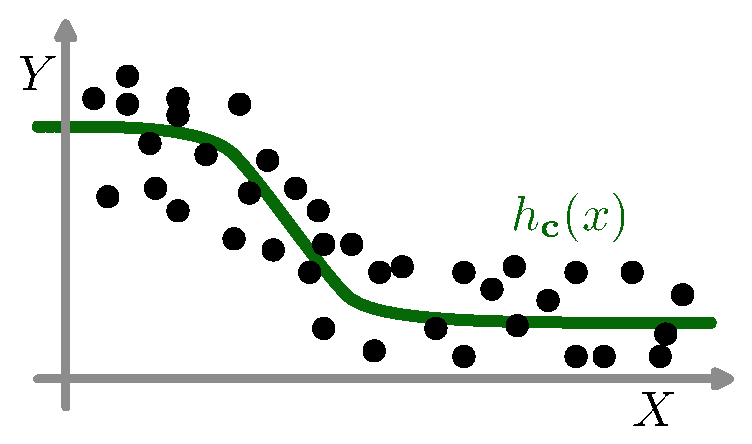
\includegraphics[width=0.95\linewidth]{chapters/mapeamento/mapeamento-hx-nonlinear.eps} 
\end{minipage}
\begin{minipage}{0.6\textwidth}
Dados,
os escalares $x \in \mathbb{R}$ e $y \in \mathbb{R}$, o vetor coluna $\VECTOR{c} \in \mathbb{R}^M$, e 
definida a Eq. (\ref{eq:maphcxr1r1:1}), 
\begin{equation}\label{eq:maphcxr1r1:1}
y=h_{\VECTOR{c}}(x)\equiv h(\VECTOR{c},x),
\end{equation}
onde $h_{\VECTOR{c}}:\mathbb{R} \rightarrow \mathbb{R}$, é uma função com dominio em $X$, contradominio em $Y$
e com coeficientes $c_m$ que formam o vetor $\VECTOR{c} \in \mathbb{R}^{M}$;
podemos afirmar que o vetor $\VECTOR{c}=\VECTOR{\hat{c}}$,
que minimiza o erro $e(\VECTOR{c})$,
\end{minipage}

\begin{equation}\label{eq:maphcxr1r1:2}
e(\VECTOR{c}) =  ||\VECTOR{h}(\VECTOR{c})-\VECTOR{y}||_{\MATRIX{W}}^2 + \alpha||\VECTOR{c}-\VECTOR{c}_{last}||_{\MATRIX{D}}^2,
\end{equation}
onde $\alpha \in \mathbb{R}$ é um multiplicador de Lagrange escolhido por nós,
\begin{equation}
\VECTOR{h}(\VECTOR{c})\equiv \VECTOR{h}_{\VECTOR{x}}(\VECTOR{c})=\begin{bmatrix}
h(\VECTOR{c},x_1)\\ 
h(\VECTOR{c},x_2)\\ 
%\vdots\\ 
%h(\VECTOR{c},x_n)\\ 
\vdots\\ 
h(\VECTOR{c},x_N)
\end{bmatrix},
~
%\VECTOR{x}=\begin{bmatrix}
%x_1\\ 
%x_2\\ 
%%\vdots\\ 
%%x_n\\ 
%\vdots\\ 
%x_N
%\end{bmatrix},
%~
\VECTOR{y}=\begin{bmatrix}
y_1\\ 
y_2\\ 
%\vdots\\ 
%y_n\\ 
\vdots\\ 
y_N
\end{bmatrix},
~
\MATRIX{W}=\funcdiag\left(\begin{bmatrix}
w_1\\ 
w_2\\ 
%\vdots\\ 
%w_n\\ 
\vdots\\ 
w_N
\end{bmatrix}\right),
~
\MATRIX{D}=\funcdiag\left(\begin{bmatrix}
d_1\\ 
d_2\\ 
%\vdots\\ 
%d_m\\ 
\vdots\\ 
d_M
\end{bmatrix}\right);
\end{equation}
pode ser achado\footnote{A demostração pode ser vista na Prova \ref{proof:theo:maphcxr1r1}.} 
usando de forma iterativa a Eq. (\ref{eq:maphcxr1r1:3})
\begin{equation}\label{eq:maphcxr1r1:3}
\VECTOR{c}_{i}=\VECTOR{c}_{i-1}-[\MATRIX{J}(\VECTOR{c}_{i-1})^{\transpose}\MATRIX{W}\MATRIX{J}(\VECTOR{c}_{i-1})+\alpha \MATRIX{D}]^{-1}\MATRIX{J}(\VECTOR{c}_{i-1})^{\transpose}\MATRIX{W}[\VECTOR{h}(\VECTOR{c}_{i-1})-\VECTOR{y}],
\end{equation}
onde a matriz $\MATRIX{J}(\VECTOR{c})$ 
$\equiv \frac{\partial \VECTOR{h}(\VECTOR{c})}{\partial \VECTOR{c}^{\transpose}}$ é a 
\hyperref[def:jacobian]{\textbf{matriz Jacobiana}}  de $\VECTOR{h}(\VECTOR{c})$,
\begin{equation}
\MATRIX{J}(\VECTOR{c})\equiv\MATRIX{J}_{\VECTOR{x}}(\VECTOR{c})=\begin{bmatrix}
\VECTOR{j}(\VECTOR{c},x_1)\\ 
\VECTOR{j}(\VECTOR{c},x_2)\\ 
%\vdots\\ 
%\VECTOR{j}(\VECTOR{c},x_n)\\ 
\vdots\\ 
\VECTOR{j}(\VECTOR{c},x_N)
\end{bmatrix},
\quad
\begin{array}{lll}
\VECTOR{j}(\VECTOR{c},x) & = & \frac{\partial h(\VECTOR{c},x)}{\partial \VECTOR{c}^{\transpose}} \\
                       ~ & ~ & ~\\
                       ~ & = & \left[\frac{\partial h(\VECTOR{c},x)}{\partial c_1}\quad \frac{\partial h(\VECTOR{c},x)}{\partial c_2}\quad ...\quad \frac{\partial h(\VECTOR{c},x)}{\partial c_{m}} \quad ... \quad \frac{\partial h(\VECTOR{c},x)}{\partial c_{M}} \right]
\end{array}
\end{equation}

\textbf{Considerações:}
\begin{itemize}
\item A busca iterativa da Eq. (\ref{eq:maphcxr1r1:3}) 
é declarada finalizada com sucesso 
quando iterações consecutivas do vetor $\VECTOR{c}_i$ convergem a valores próximos, onde declaramos $\VECTOR{\hat{c}}=\VECTOR{c}_i$.
\item O erro mínimo, $e(\VECTOR{\hat{c}}) \geq 0$, não necessariamente ter valor zero. 
\end{itemize}
\end{theorem}

%\begin{tcbattention}
%\begin{itemize}
%\item 
%\end{itemize}
%\end{tcbattention}

%%%%%%%%%%%%%%%%%%%%%%%%%%%%%%%%%%%%%%%%%%%%%%%%%%%%%%%%%%%%%%%%%%%%%%%%%%%%%%%%
\subsection{Exemplos de mapeamento usando uma função
$h(\VECTOR{c},x):~\mathbb{R} \rightarrow \mathbb{R}$}

\begin{example}\label{ex:theo:maphcxr1r1}
Conhecida as $N=18$ amostras $x_n$ e $y_n$, mostradas nas  Tabelas \ref{table:theo:maphcxr1r1:xn} e \ref{table:theo:maphcxr1r1:yn},
achar os parametros $c_m$ do vetor $\VECTOR{c}=[c_1\quad c_2\quad c_3]^{\transpose}$ da função $h(\VECTOR{c},x)$, 
\begin{equation}
h(\VECTOR{c},x)=c_1 e^{-\left(\frac{x}{c_2}\right)^{-4}}+c_3,
\end{equation}
que gere o menor erro 
$e(\VECTOR{c})=0.1 ||\VECTOR{c}-\VECTOR{c}_{last}||^2 + \sum_{n=1}^{N} ||h(\VECTOR{c},x_n)-y_n||^2 $.
\end{example}


\begin{table}[h!]
\centering
\begin{tabular}{|c|c|c|c|c|c|c|c|c|} 
 \hline
$n$   & 1 & 2 & 3 & 4 & 5 & 6 & 7 & 8\\ \hline
$x_n$ & 0.10461 & 0.29614 & 1.63968 & 1.89586 & 3.17301 & 3.68811 & 3.75758 & 3.96560 \\ \hline
 \hline
$n$   & 9 & 10 & 11 & 12 & 13 & 14 & 15 & 16\\  \hline
$x_n$ & 6.09526 & 6.12999 & 6.81288 & 8.33457 & 8.74851 & 8.81418 & 9.16269 & 9.30314 \\ \hline
\end{tabular}
\caption{Valores $x_n$.}
\label{table:theo:maphcxr1r1:xn}
\end{table}

\begin{table}[h!]
\centering
\begin{tabular}{|c|c|c|c|c|c|c|c|c|} 
 \hline
$n$   & 1 & 2 & 3 & 4 & 5 & 6 & 7 & 8\\ \hline
$y_n$ & 9.9005 & 10.1155 & 9.3351 & 8.7244 & 4.4788 & 3.0054 & 2.4827 & 2.3804  \\ \hline
 \hline
$n$   & 9 & 10 & 11 & 12 & 13 & 14 & 15 & 16\\  \hline
$y_n$ & 1.7806 & 2.1098 & 1.9972 & 1.8630 & 2.2316 & 1.8932 & 2.0231 & 2.2066 \\ \hline
\end{tabular}
\caption{Valores $y_n$.}
\label{table:theo:maphcxr1r1:yn}
\end{table}

\begin{SolutionT}[Relativa ao Exemplo \ref{ex:theo:maphcxr1r1}:]\label{sol:theo:maphcxr1r1}
Para obter  o vetor $\VECTOR{c}=\VECTOR{\hat{c}}$, da função $h(\VECTOR{c},x) = c_1~ e^{-\left(\frac{x}{c_2}\right)^{-4}}+c_3$,
%\begin{equation}
%h(\VECTOR{c},x)=c_1~ e^{-\left(\frac{x}{c_2}\right)^{-4}}+c_3,
%\end{equation} 
com o menor erro $e(\VECTOR{c})=0.1 ||\VECTOR{c}-\VECTOR{c}_{last}||^2 + \sum\limits_{n=1}^{N} ||h(\VECTOR{c},x_n)-y_n||^2 $,
podemos usar iterativamente a Eq. (\ref{eq:maphcxr1r1:3}), com 
\begin{equation}
\frac{\partial h(\VECTOR{c},x)}{\partial c_1} 
= e^{-\left(\frac{x}{c_2}\right)^{-4}},\qquad 
\frac{\partial h(\VECTOR{c},x)}{\partial c_2} 
= 4\frac{c_1}{c_2}\left(\frac{x}{c_2}\right)^{-4}e^{-\left(\frac{x}{c_2}\right)^{-4}}, \qquad 
\frac{\partial h(\VECTOR{c},x)}{\partial c_3} 
=1
\end{equation} 
iniciando desde um vetor $\VECTOR{c}_{0}=[1\quad 1\quad 1]^{\transpose}$ escolhido arbitrariamente.
Obtendo assim a Tabela \ref{table:theo:maphcxr1r1:ei}, que conclui em
$\VECTOR{\hat{c}}=\VECTOR{c}_{5}=[7.9767\quad 3.0212\quad 2.0039]^{\transpose}$,
com  um erro $e(\VECTOR{c}_{5})=0.31848$.


\begin{table}[h!]
\centering
\begin{tabular}{|c|c|c|c|c|c|c|} 
 \hline
$i$   & 0 & 1 & 2 & 3 & 4 & 5 \\ \hline
\hline
$c_1$ & 1.0000 & 6.4006 & 7.5254 & 7.9571 & 7.9759 & 7.9767 \\ \hline
$c_2$ & 1.0000 & 2.3743 & 3.0158 & 3.0210 & 3.0212 & 3.0212 \\ \hline
$c_3$ & 1.0000 & 3.3416 & 2.2483 & 2.0111 & 2.0042 & 2.0039 \\ \hline
\hline
$e(\VECTOR{c}_{i})$ & 286.15891 & 19.10286 & 1.05792 & 0.31951 & 0.31848 & 0.31848  \\ \hline
\end{tabular}
\caption{Valores $e(\VECTOR{c}_{i})$ e vetores $\VECTOR{c}_{i}$.}
\label{table:theo:maphcxr1r1:ei}
\end{table}

    \begin{figure}[!h]
        \centering
        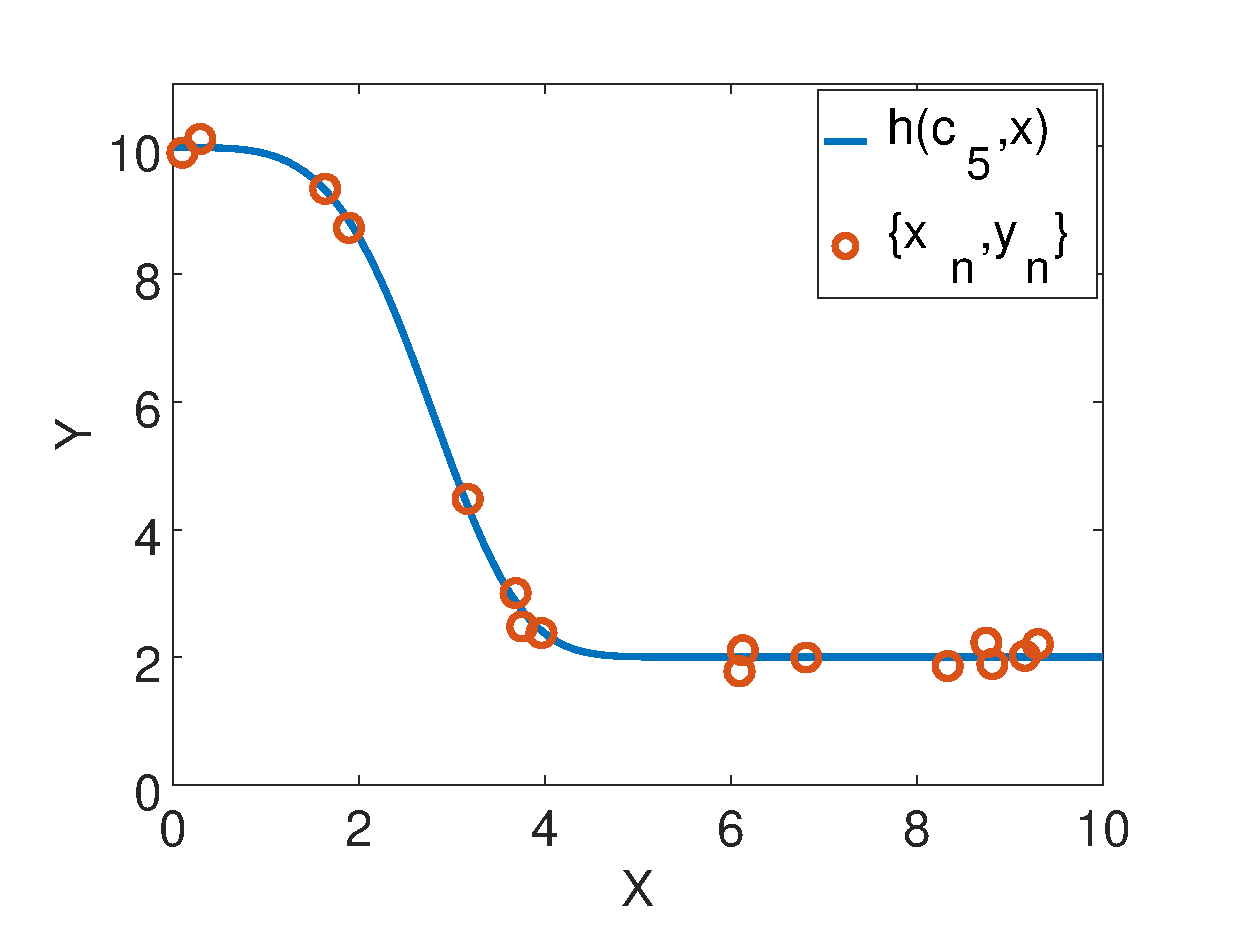
\includegraphics[width=0.49\textwidth]{chapters/mapeamento/mfiles/mapeamentor1r1-nonlinear/minimizando_hx.eps}
        \caption{Gráfico das amostras $\{x_n,y_n\}$ e da curva $x$ vs. $h(\VECTOR{c}_5,x)$.}
        \label{fig:theo:maphcxr1r1:xnyn}
    \end{figure}

\end{SolutionT}


